\chapter{Numerical Methods and Implementation}
\label{chap:num}
%The governing equations having been derived in~\Cref{chap:governing}, the next step is to choose a suitable \textit{discretization method}, which approximates these differential equations into a system of algebraic equations.
In this chapter the discretization methods which approximate the differential equations established in Chapter 2 are presented.
The discretization methods used in both NX Flow and syn3D is the finite volume (FV) method, which is described in~\Cref{sec:fv} in a general sense. Methods of calculating the wall distance are discussed in~\Cref{sec:walldist}. \Cref{sec:syn3d,sec:nxflow} discuss the specifics of the implementation and chosen numerical schemes for syn3D and NX Flow respectively.
%
%
\section{Finite Volume Method}
\label{sec:fv}
%
%
The finite volume method requires the specification of a \textit{computational grid}, a discrete representation of the geometric domain on which the problem is to be solved. Another name for computational grid is \textit{mesh}. This essentially divides the domain into a finite number of subdomains. In the case of the finite volume method, these subdomains are referred to as \textit{control volumes} (CVs). The governing equations must then be solved over each of these discrete control volumes, which results in a solution field at discrete locations, as opposed to an analytic function.

\subsection{Integral form of the conservation laws}
A special property of the finite volume method is that it uses the integral form of the conservation equations. Moreover, it employs the Gauss theorem, also known as divergence theorem, to express volume integrals as surface integrals. Specifically, let $\vec{F}$ be a continuously differentiable vector field, $\vol$ be a volume in three-dimensional space, $\surf$ be the boundary of the volume and $\text{d}S$ be a surface element along with its associated unit outward normal vector $\vec{n}$, the divergence theorem states that:
\begin{equation*}
    \iiint_{\vol} \left( \nabla \cdot \vec{F} \right)~d\vol =
        \oiint_{\surf} (\vec{F}\cdot\vec{n})~dS.
\end{equation*}
The integral on the left-hand side is a volume integral, whereas the integral on the right-hand side is a surface integral. For the remainder of this work, the triple integral and closed integral notations will be replaced with simple integrals, where the type can be inferred from the limit ($\vol$ or $\surf$).

Investigation of~\Cref{eq:mass,eq:mom,eq:energy} reveals commonalities between the equations. Again, let $\phi$ be a general conserved property, the so-called transport equation for $\phi$ can be written in integral form as:
\begin{equation}
    \pdiff{}{t}\int_\vol \rho \phi~d\vol
        + \int_{\surf} (\rho \phi \vec{u})\cdot\vec{n}~dS
        = \int_{\surf} (\Gamma \nabla \phi)\cdot\vec{n}~dS
        + \int_\vol Q_\phi~d\vol
    \label{eq:fvtransport},
\end{equation}
where $\Gamma$ is a general diffusion coefficient and $Q_\phi$ is the source term. Reading from left to right, the terms are labelled as: temporal derivative term, convective term, diffusive term and source term. The convective and diffusive terms being surface integrals, are also referred to as \textit{flux} terms. All conservation equations, specifically mass, momentum and energy, can be written in this form, where $Q$ takes care of the special terms, e.g. the pressure gradient term in the momentum equation.

The finite volume method is attractive due to its simplicity and its ability to accommodate any type of grid. The method is also \textit{conservative} by construction, so long as fluxes for CVs sharing a boundary are identical.

Again,~\Cref{eq:fvtransport} is to be solved over all CVs. Within each CV lies a \textit{computational node}, also known as field point, at which the dependent quantities are to be calculated.
%
%
\subsection{Numerical approximations}
\label{sec:fvnum}
%
%
The integral transport equation in~\Cref{eq:fvtransport} remains analytical; no numerical approximations have been made thus far. To enable computer implementation, the equation must be discretized, so as to yield a finite set of algebraic equations in the form of:
\begin{equation*}
    a_P \phi_P + \sum_{nb}a_{nb}\phi_{nb} = b_P,
\end{equation*}
where $P$ is the control volume of interest, $a$'s and $b$'s are constant coefficients, and $nb$ represents the neighboring field points involved in the discretization. One speaks of a \textit{stencil} when referring to these neighbors. Discretization inevitably introduces discretization errors, which is why it is always an approximation. The goal is to reduce these errors to a negligible level.

Discretization of the finite volume equations can be split in two steps:
\begin{description}
    \item[Spatial discretization]: Numerical approximation of integrals and spatial derivatives
    \item[Temporal discretization]: Numerical approximation of time derivative
\end{description}

\subsubsection{Spatial discretization}
Every term in~\Cref{eq:fvtransport} is an integral. To calculate either the volume or surface integrals exactly would require knowledge of the integrand everywhere on the volume or surface; however such information is not available. Discretization of the integrals in~\Cref{eq:fvtransport} can be done using three levels of approximation: integration, interpolation and differentiation.

Let $\vec{F}$ be a flux vector, the closed surface integrals for an arbitrary polyhedron, which is the only type of three-dimensional control volume that is used in most finite volume codes, then the integral of the normal flux over the control surface can be written as:
\begin{equation}
    \int_{\surf} (\vec{F}\cdot \vec{n})~dS = \sum_{k=1}^{N_f} \int_{S_k} (\vec{F}\cdot\vec{n}_k)~dS
    \label{eq:surfint},
\end{equation}
where $N_f$ is the number of faces. Taking for instance a hexahedron, a commonly used element in CFD, like the one depicted in~\Cref{fig:hex}, the closed integral is simply the sum of the integral over all $N_f = 6$ faces.

The individual face integrals then need to be numerically integrated. The most commonly used numerical integration method (quadrature) is the midpoint rule, for which there is only one integration point placed at the face center. Application of the midpoint rule to a single surface integral in~\Cref{eq:surfint} yields:
\begin{equation*}
   \int_{S} \vec{F}\cdot\vec{n}~dS = (\vec{F}_{S_c}\cdot\vec{n}) S + \order(\delta^2),
\end{equation*}
where $S$ is the surface area, $\vec{F}_{S_c}$ is $\vec{F}$ evaluated at the face center and $\delta$ is the characteristic length.  The approximation is of second-order accuracy, as denoted by the second term on the right-hand side, provided that $\vec{F}_{S_c}$ is also evaluated with at least second-order accuracy. Then, a closed surface integral may be written as a sum over all integration points ($ip$)
\begin{equation*}
    \int_{\surf} (\vec{F}\cdot\vec{n})~dS = \sum_{ip} (\vec{F}_{ip}\cdot\vec{n}_{ip}) S_{ip}.
\end{equation*}

The volume integral can also be numerically integrated using the midpoint rule. A volume integral over a CV can then be approximated as:
\begin{equation*}
    \int_\vol G~d\vol = G_{P} V + \order(\delta^2),
\end{equation*}
where $V$ is the volume and $G_{P}$ is $G$ at the field point $P$. This method is of second-order accuracy provided that $P$ lies at the CV centroid.

Application of the integral approximations to~\Cref{eq:fvtransport}, ignoring the $\order$ terms, results in:
\begin{equation}
    \pdiff{(\rho\phi V )_P}{t}
    =
    \sum_{ip} [-(\rho\phi\vec{u})_{ip}\cdot\vec{n}_{ip}] S_{ip}
    = \sum_{ip} [(\Gamma\nabla\phi)_{ip}\cdot\vec{n}_{ip}] S_{ip}
    + Q_P V
    \label{eq:spatial}.
\end{equation}

Whereas all quantities at point $P$ are readily available, quantities and gradients at the integration points must be expressed in terms of the field point values via interpolation and differentiation schemes respectively. Interpolation and differentiation schemes are discussed for each solver separately.

\subsubsection{Temporal discretization}
Application of spatial discretization schemes leads to an ordinary differential equation (ODE) for each CV of the form:
\begin{equation}
    \pdiff{(\rho\phi V)_P}{t} = R_P
    \label{eq:temp1},
\end{equation}
where $R$ is the so-called residual of the equation and generally includes quantities depending on neighboring field points.

Given the solution field $\phi^n$ at time $t$, a new solution $\phi^{n+1}$ at time $t + \Delta t$ is sought. This is typically done even for steady-state problems using the concept of pseudo-time~\cite{blazek2015computational}, which is necessary due to the non-linearity of the equations. Integrating in time on both sides of~\Cref{eq:temp1} results in:
\begin{equation}
    \int_t^{t+\Delta t}
        \pdiff{(\rho \phi V)_P}{t}
   ~dt
    = -\int_t^{t+\Delta t} R_P~dt
    \label{eq:time2}.
\end{equation}
Since the only unknown field in this equation is $\phi$, it is possible to say:
\begin{equation*}
    \pdiff{(\rho \phi V)_P}{t} = (\rho V)_P \pdiff{\phi_P}{t}.
\end{equation*}
The left-hand side \Cref{eq:time2} can then be evaluated as:
\begin{equation}
    \int_t^{t+\Delta t}
        \pdiff{(\rho \phi V)_P}{t}
   ~dt =
   (\rho V)_P (\phi^{n+1} - \phi^n)_P
   = (\rho V)_P \Delta \phi_P^n
   \label{eq:timediff}.
\end{equation}
Integration of the right-hand side of~\Cref{eq:time2} can be done in various ways: one can use the solution at time $t$, time $t + \Delta t$ or a mix of both to calculate the integral. Certain codes even use the solution at time $t - \Delta t$, although this is not done in either solver presented in this work.  A family of methods can be generalized by introducing a weighting parameter $\theta$ which is allowed to vary between 0 and 1 and approximating the integral of the residual as:
\begin{equation}
    \int_t^{t+\Delta t} R_P~dt = \left[
        \theta R_P^{n+1} + (1 - \theta) R_P^n
    \right] \Delta t
    \label{eq:timeint}.
\end{equation}
The forward Euler, backward Euler and Crank-Nicolson methods can be recovered by letting $\theta = 0$, $\theta = 1$ and $\theta = 0.5$ respectively. Substitution of~\Cref{eq:timediff,eq:timeint} in~\Cref{eq:time2} and dividing by $\Delta t$ on both sides results in:
\begin{equation}
    \frac{(\rho V)_P}{\Delta t}\Delta \phi_P^n = -\theta R_P^{n+1} - (1 - \theta) R_P^n
    \label{eq:timeimp}.
\end{equation}
Evaluation of $R_P^{n+1}$ in~\Cref{eq:timeimp} requires knowledge of the solution field at the new time level $\phi^{n+1}$, which is not known a priori. To complicate matters, the residual in the Navier-Stokes equations is non-linear and its discretized form cannot be expressed as a linear combination of the field points. However, it is possible to linearise the residual at the new time level with a first-order Taylor series expansion:
\begin{equation*}
    R_P^{n+1} \approx R_P^n + \left(\pdiff{R}{\phi}\right)_P \Delta \phi_P^n,
\end{equation*}
where the partial differential term $\partial R/\partial \phi$ is commonly referred to as the flux Jacobian and depends on the chosen spatial discretization schemes. Substituting the linearisation in~\Cref{eq:timeimp} results in:
\begin{equation}
    \left[
        \frac{(\rho V)}{\Delta t} + \theta \left(\pdiff{R}{\phi}\right)
    \right]_P \Delta \phi_P^n
    = -R_P^n.
\end{equation}
Thus, provided an initial solution field, it is possible to advance $\phi$ in pseudo-time until the solution is \emph{converged}, i.e. a steady-state solution is reached. Convergence is typically monitored by calculating $||R||_k$ where $k$ is a specified vector norm, which is typically either the Euclidean norm or the infinity norm. A converged solution is then attained when the norm of the residual falls below a user-specified tolerance $\epsilon$.

Regardless of the chosen scheme, the result is a linear system of equations of the familiar form:
\begin{equation*}
    Ax = b,
\end{equation*}
where $A$ is a sparse matrix, $x$ is the vector of unknowns and $b$ is a vector. The linear system can be solved with a direct or iterative method.

\section{Wall distance computation methods}
\label{sec:walldist}
Calculation of the wall distance $d$ is required in order to solve the Spalart-Allmaras equation. In the literature, it is typically computed in one of two ways:
\begin{enumerate}
    \item by a brute force approach.
    \item by solving an additional PDE.
\end{enumerate}
The brute force approach is straight-forward and consists of looping through every CV and finding the nearest wall, which itself is done by looping over every face lying on the solid boundary. Depending on the mesh, this approach can be very costly~\cite{tucker2005computations}. Moreover, some codes approximate the wall distance for a field point $P$ as the distance between $P$ and the nearest node or face center lying on a solid boundary, as opposed to calculating the perpendicular distance between a point and a plane, which is more costly. This approximation and the potential error are illustrated in~\Cref{fig:nasawalldist}.
\begin{figure}
    \centering
    \includegraphics[width=0.55\textwidth]{figs/mindist}
    \caption{Common approximation made in brute force wall distance calculations~\cite{tmr}.}
    \label{fig:nasawalldist}
\end{figure}

The other approach, solving an additional PDE, may seem like a lot of extra work. However, CFD codes already provide functions and data structures required in solving such equations. There exists many different equations for approximating the wall distance, which are detailed and compared in~\cite{tucker2005computations,tucker2011hybrid,belyaev2015variational}. The technique used in syn3D and NX Flow consists of solving a Poisson equation followed by a normalization, which can mathematically be written as:
\begin{align}
    \begin{split}
    \nabla^2\phi &= -1\\
    d &= ||\nabla\phi||_2 + \sqrt{
        ||\nabla\phi||_2 + 2\phi
    }
    \end{split}
    \label{eq:poissondist}.
\end{align}
A homogeneous Dirichlet BC is to be imposed on $\phi$ at solid walls and a homogeneous Neumann BC at all other boundaries. The approximation of $d$ by~\Cref{eq:poissondist} is only accurate close to walls, however that is the only location where an accurate $d$ is needed when it comes to turbulence modelling.

\section{Syn3D}
\label{sec:syn3d}
%
%
The academic code, named syn3D, is owned by Professor Siva Nadarajah of McGill University. The program has the following characteristics:
\begin{itemize}
    \item Non-dimensional
    \item Structured
    \item Uses coordinate transformation to generalized curvilinear coordinates
    \item Cell-centered
\end{itemize}
Non-dimensionalization is explained in~\Cref{syn:nondim}, the mesh structure is given in~\Cref{sec:synmesh}, the coordinate transformation method is summarized in~\Cref{sec:transform}, the discretization of the fluid flow and turbulence governing equations are given in~\Cref{sec:synns,sec:synturb} respectively and the wall distance calculation details are given in~\Cref{sec:synwalldist}.
%
\subsection{Non-dimensionalization}
\label{syn:nondim}
%
Round-off errors can be reduced by non-dimensionalizing the governing equations such that all quantities remain in the same order of magnitude. While arbitrary reference quantities can be used, it is convenient to use significant quantities. External flow problems being usually described by free-stream values, the following scaling parameters are used: the airfoil chord length $L$, the free-stream density $\rho_\infty$, the free-stream pressure $p_\infty$, the free-stream dynamic viscosity $\mu_\infty$ and a reference temperature $T_{ref}$. Usage of these scales leads to the following relations between dimensional quantities, now denoted by the superscript $^*$, and non-dimensionalized quantities:
\begin{gather*}
    \rho = \frac{\rho^*}{\rho_\infty}, \quad\quad
    u_i = \frac{u_i^*}{\sqrt{p_\infty/\rho_\infty}}, \quad\quad
    p = \frac{p^*}{p_\infty}, \quad\quad
    i = \frac{i^*}{p_\infty/\rho_\infty}, \\
    x_i = \frac{x_i^*}{L}, \quad\quad
    t = \frac{t^*\sqrt{p_\infty/\rho_\infty}}{L}, \quad\quad
    \Omega = \Omega^*\frac{c}{\sqrt{p_\infty/\rho_\infty}}, \\
    \mu = \frac{\mu^*}{\mu_\infty}, \quad\quad
    \mu_T = \frac{\mu^*_T}{\mu_\infty}, \quad\quad
    \sa = \frac{\sa^*}{\mu_\infty/\rho_\infty}, \quad\quad
    d = \frac{d^*}{L}.
\end{gather*}
It also should be noted that the dynamic viscosity is computed from the temperature using Sutherland's law
\begin{equation*}
    \mu = \frac{C_1 T^{3/2}}{T + S},
\end{equation*}
where $C_1 = 1.461E-6$, $S = 110.3$. The temperature in the previous equation is computed from
\begin{equation*}
    T = T_{ref} \frac{p}{\rho},
\end{equation*}
The free-stream dynamic viscosity is computed in the same manner using $T_{ref}$ in the place of $T$.

Substitution of the non-dimensional relations into~\Cref{eq:fansmass,eq:fansmom,eq:fansenergy}, the Favre-averaged Navier-Stokes equations, and rearranging yields:
\begin{align}
    \Dphi{} &= 0 \\
    \pdiff{\rho\vec{u}}{t}
    + \nabla\cdot(\rho\vec{u}\otimes\vec{u})
    &= -\nabla p + \ndim\nabla\cdot(\tau + \tau^T)
    \\
    \pdiff{\rho E}{t} + \nabla\cdot (\rho \vec{u} H) &=
        \ndim\nabla\cdot \left[
            (\tau + \tau^T) \cdot \vec{u}
        \right]
        - \ndim\nabla\cdot\left(k_{\text{eff}}\nabla T\right) .
\end{align}
The equations are unchanged except for the additional scaling factor $\ndim$ multiplying viscous terms in the momentum and energy equations, where $M_\infty$ is the free-stream Mach number. This also shows that an increase in the Reynolds number will cause a decrease of the viscous forces, which is in agreement with the definition of the Reynolds number.

Repeating the process above for the Spalart-Allmaras equation and rearranging the production and destruction terms so as to group terms with common factors results in:
\begin{align}
\begin{split}
    \pdiff{\sa}{t} + \vec{u}\cdot(\nabla\sa) &=
        c_{b1}(1 - f_{t2})\Omega\sa
        + \ndim \left\{
            C_{b1}[(1 - f_{t2})f_{v2} + f_{t2}]\frac{1}{\kappa^2} - c_{w1}f_w
        \right\} \left(\frac{\sa}{d}\right)^2
        \\
        &+ \ndim \frac{1}{\sigma}\nabla\cdot\left[ (\nu + \sa) \nabla\sa \right]
        + \ndim \frac{c_{b2}}{\sigma}\left(\nabla \sa\right)^2.
\end{split}
\label{eq:synsa}
\end{align}
The auxiliary functions require the same treatment:
\begin{gather*}
    r = \text{min} \left[
        \ndim \frac{\sa}{\hat{S}\kappa^2 d^2}, 10
    \right] \\
    \hat{S} = \Omega + \ndim \frac{\sa}{\kappa^2 d^2} f_{v2}.
\end{gather*}
Unmentioned functions as well as constants remain unchanged.
\label{sec:synnondim}
%
\subsection{Computational Grid}
%
\label{sec:synmesh}
Syn3D solves problems on three-dimensional multiblock-structured meshes, making the hexahedron the only acceptable element type. Moreover, a field point is located at the centroid of each element -- it follows that the CVs are all hexahedrons. A general hexahedron CV is shown in~\Cref{fig:hex}. In structured grids, each field point, or CV, is uniquely identified by its $i$, $j$ and $k$ indices. Its neighbors can also be identified by incrementing and decrementing the $i$, $j$ and $k$ indices, which is the main advantage of this method.
%This is illustrated in~\Cref{fig:structured} for the two-dimensional case, where elements are instead quadrilaterals.
A more detailed discussion of grid generation is given in~\cite{blazek2015computational}.
\begin{figure}
\centering
    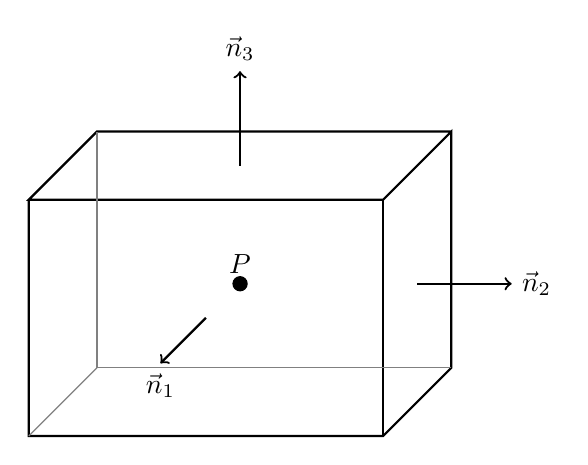
\begin{tikzpicture}[scale=1.5]
  \pgfmathsetmacro{\dx}{3}
  \pgfmathsetmacro{\dy}{2}
  \pgfmathsetmacro{\dz}{1.5}
  \draw[thick](\dx,\dy,0)--(0,\dy,0)--(0,\dy,\dz)--(\dx,\dy,\dz)--(\dx,\dy,0)--(\dx,0,0)--(\dx,0,\dz)--(0,0,\dz)--(0,\dy,\dz);
  \draw[thick](\dx,\dy,\dz)--(\dx,0,\dz);
  \draw[gray](\dx,0,0)--(0,0,0)--(0,\dy,0);
  \draw[gray](0,0,0)--(0,0,\dz);
  \draw[fill] (\dx*0.5, \dy*0.5, \dz*0.5) circle [radius=\dx*0.02] node [above] {$P$};
  \draw[->,thick] (0.5*\dx,0.5*\dy,\dz)
    %node {$\times$}
    -- (0.5*\dx,0.5*\dy,\dz+1) node [below] {$\vec{n}_1$};
  \draw[->,thick] (\dx,0.5*\dy,0.5*\dz)
    %node {$\times$}
    -- (\dx+0.8,0.5*\dy,0.5*\dz) node [right] {$\vec{n}_2$};
  \draw[->,thick] (0.5*\dx,\dy,0.5*\dz)
    %node {$\times$}
    -- (0.5*\dx,\dy+0.8,0.5*\dz) node [above] {$\vec{n}_3$};
  %\node at (0.5*\dx, 0.5*\dy, 0.0) {$\times$};
  %\node at (0.0, 0.5*\dy, 0.5*\dz) {$\times$};
  %\node at (0.5*\dx, 0.0, 0.5*\dz) {$\times$};
  % \draw[
  %\node [align=left] at (0.0, -\dy*0.3, \dz) {
    %\begin{tabular}{cl}
   % $\times$ & Integration point\\
    %\tikz\draw[fill] circle (0.5ex); & Field point
    %\end{tabular}
%};
\end{tikzpicture}
\caption{A hexahedron element. Field point is shown as solid black circle.}\label{fig:hex}
\end{figure}

%\begin{figure}
%\centering
%\begin{tikzpicture}
%  % Use https://www.easycalculation.com/area/polygon-centroid-point.php for centroid
\begin{tikzpicture}[scale=5.0]
  % I lines
  \draw (-0.05,-0.02) -- (0.0,0.0) -- (0.7, 0.03) -- (1.5, 0.0) -- (2.2, 0.0) -- (2.25, -0.02);
  \draw (0.05,0.6) -- (0.1, 0.7) -- (0.68, 0.72) -- (1.53, 0.62) -- (2.15, 0.60) -- (2.2, 0.61);
  \draw (0.0, 1.2) -- (0.05, 1.21) -- (0.83, 1.28) -- (1.58, 1.2) -- (2.2, 1.18) -- (2.25, 1.19);
  \draw (0.03, 1.7) -- (0.08, 1.70) -- (0.77, 1.65) -- (1.5, 1.67) -- (2.12, 1.7) -- (2.17, 1.72);
  % J lines
  \draw (-0.02, -0.05) -- (0.0,0.0) -- (0.1, 0.7) -- (0.05, 1.21) -- (0.08, 1.70) -- (0.06, 1.75);
  \draw (0.79, -0.02) -- (0.7, 0.03) -- (0.68, 0.72) -- (0.83, 1.28) -- (0.77, 1.65) -- (0.79, 1.7);
  \draw (1.49, -0.05) -- (1.5, 0.0) -- (1.53, 0.62) -- (1.58, 1.2) -- (1.5, 1.67) -- (1.52, 1.72);
  \draw (2.19, -0.05) -- (2.2, 0.0) -- (2.15, 0.60) -- (2.2, 1.18) -- (2.12, 1.7) -- (2.11, 1.75);
  % Field points
\draw[fill] (0.370, 0.362) circle [radius=0.02] node [above] {i-1, j-1};
\draw[fill] (0.415, 0.978) circle [radius=0.02] node [above] {i-1, j    };
\draw[fill] (0.432, 1.460) circle [radius=0.02] node [above] {i-1, j+1};
\draw[fill] (1.103, 0.343) circle [radius=0.02] node [above] {i    , j-1};
\draw[fill] (1.155, 0.955) circle [radius=0.02] node [above] {i    , j    };
\draw[fill] (1.170, 1.450) circle [radius=0.02] node [above] {i    , j+1};
\draw[fill] (1.845, 0.305) circle [radius=0.02] node [above] {i+1, j-1};
\draw[fill] (1.865, 0.900) circle [radius=0.02] node [above] {i+1, j    };
\draw[fill] (1.850, 1.438) circle [radius=0.02] node [above] {i+1, j+1};
\end{tikzpicture}
%\end{tikzpicture}
%\caption{Part of a two-dimensional structured grid}
%\label{fig:structured}
%\end{figure}
%
%\subsection{Numerical schemes}
%\label{sec:synnum}
%


%Spatial discretization, temporal discretization and boundary conditions are described in~\Cref{sec:synspace,sec:syntemp,sec:synbc} respectively.
%
\subsection{Coordinate transformation}
\label{sec:transform}
%
%Usage of a structured grid allows Syn3D to use certain numerical schemes that would not be possible to use with unstructured grids. More specifically, it is possible to write the
The governing equations are written in generalized curvilinear coordinates through a transformation from physical space (Cartesian coordinates) to a more convenient computational space (generalized curvilinear coordinates). A curvilinear grid can be represented through a transformation from the Cartesian coordinates $x_i$ ($x$, $y$, $z$ in three dimensions) to curvilinear coordinates $\xi_i$ ($\xi$, $\eta$, $\zeta$ in three dimensions), where each grid line is a line of constant coordinate $\xi_i$. In three dimensions, $\xi$, $\eta$ and $\zeta$ correspond to the index-directions $i$, $j$, $k$ mentioned in~\Cref{sec:synmesh}. \Cref{fig:transformation} illustrates the concept in two dimensions. The transformation is performed by setting the new coordinates to be functions of the Cartesian coordinates, and vice versa:
\begin{equation*}
    \xi_i = \xi_i(x_j), \quad x_i = x_i(\xi_j), \quad j=1,2,3.
\end{equation*}
\begin{figure}
    \centering
    \begin{tikzpicture}
    %   % http://texample.net/tikz/examples/polar-plot/
% https://tex.stackexchange.com/questions/330580/drawing-a-semicircle-in-tikz
% https://tex.stackexchange.com/questions/66216/draw-arc-in-tikz-when-center-of-circle-is-specified


% Computational
\def\centerarc[#1](#2)(#3:#4:#5)% Syntax: [draw options] (center) (initial angle:final angle:radius)
    { \draw[#1] ($(#2)+({#5*cos(#3)},{#5*sin(#3)})$) arc (#3:#4:#5); }
    
\foreach \rad in {2,2.5,...,4} {
    \centerarc[](0,0)(90:180:\rad);
}
\foreach \ang in {0,...,7} {
    \draw (\ang*90/7 + 90:2) -- (\ang*90/7 + 90: 4);
}
\node[below] at (180:3) {A};
\node[below right] at (135:2) {B};
\node[right] at (90:3) {C};
\node[above left] at (135:4) {D};

% CSYS
\draw [thick, <->] (0,0.5) node [left] {$y$}
-- (0,0) -- (0.5,0) node [below right] {$x$};


\draw [very thick, ->] (1, 2) -- (2, 2);

\def\xin{3}
\def\xf{6.5}
\def\yin{0.5}
\def\yf{4}
\def\ni{7}
\def\nj{4}
\pgfmathsetmacro{\ys}{(\yf - \yin)/(\nj)}
\pgfmathsetmacro{\xs}{(\xf - \xin)/(\ni)}
\foreach \y in {0,...,\nj} {
    \draw (\xin,\y*\ys + \yin) -- (\xf,\y*\ys + \yin);
}
\foreach \x in {0,...,\ni} {
    \draw (\x*\xs + \xin,\yin) -- (\x*\xs + \xin,\yf);
}
\node[left]  at (\xin,0.5*\yf + 0.5*\yin) {A};
\node[right] at (\xf, 0.5*\yf + 0.5*\yin) {C};
\node[below] at (0.5*\xf + 0.5*\xin,\yin) {B};
\node[above] at (0.5*\xf + 0.5*\xin, \yf) {D};

\draw[very thick] (\xin,\yin-0.1) -- (\xin,\yin-0.4) node [below] {\footnotesize $\text{i}=1$};
\draw[very thick] (\xf,\yin-0.1) -- (\xf,\yin-0.4) node [below] {\footnotesize ~~~~$\text{i}= \text{i}_{\text{max}}$};

\draw[very thick] (\xf+0.1,\yin) -- (\xf+0.4,\yin) node [right] {\footnotesize $\text{j}=1$};
\draw[very thick] (\xf+0.1,\yf) -- (\xf+0.4,\yf) node [right] {\footnotesize $\text{j}= \text{j}_{\text{max}}$};

\draw[thick, <->] (9,0.5) node [left] {$\eta$}
    -- (9,0) -- (9.5,0) node [below right] {$\xi$};
    \end{tikzpicture}
    \caption{Mapping from physical space ($x$, $y$) to computational space ($\xi$, $\eta$)}
    \label{fig:transformation}
\end{figure}

Transformation from physical to computational space is then defined by the metrics:
\begin{equation*}
    K_{nm} = \left[ \pdiff{x_n}{\xi_m} \right], \quad
    J = \text{det}(K), \quad
    K_{nm}^{-1} = \left[ \pdiff{\xi_n}{x_m} \right], \quad n,m = 1, 2, 3.
\end{equation*}

Cartesian derivatives can then be expressed in terms of the curvilinear coordinates using the chain rule:
\begin{equation}
    \pdiff{\phi}{x_j} = K_{ij}^{-1}\pdiff{}{\xi_i},
    \label{eq:transform}
\end{equation}
where implicit summation is used.

A geometrical interpretation of these metric terms can be made. The Jacobian $J$ corresponds to the volume of the cell and the vector $\nabla \xi_k J$ is the directed area of the cell interface normal to the $\xi_k$ direction. The following notation can then be introduced
\begin{gather*}
    \nabla \xi_k J = \vec{S}_k = (S_{k1}, S_{k2}, S_{k3}) \\
    \frac{\vec{S}_k}{|\vec{S}_k|}= \vec{n},
\end{gather*}
where the $\vec{n}$ for the face in the $\xi_k$ direction is chosen and in this case $\vec{n}$ always points towards increasing $\xi_k$.

% \begin{equation}
%     \begin{pmatrix}
%         \pdiff{}{x} \\
%         \pdiff{}{y} \\
%         \pdiff{}{z}
%     \end{pmatrix}
%     =
%     \begin{pmatrix}
%         \pdiff{\xi}{x} & \pdiff{\eta}{x} & \pdiff{\zeta}{x} \\
%         \pdiff{\xi}{y} & \pdiff{\eta}{y} & \pdiff{\zeta}{y} \\
%         \pdiff{\xi}{z} & \pdiff{\eta}{z} & \pdiff{\zeta}{z}
%     \end{pmatrix}
%     \begin{pmatrix}
%         \pdiff{}{\xi} \\
%         \pdiff{}{\eta} \\
%         \pdiff{}{\zeta}
%     \end{pmatrix}
%     \label{eq:transform1}
% \end{equation}
% One can also write the inverse transformation in matrix form:
% \begin{equation}
%     \begin{pmatrix}
%         \pdiff{}{\xi} \\
%         \pdiff{}{\eta} \\
%         \pdiff{}{\zeta}
%     \end{pmatrix}
%     =
%     \begin{pmatrix}
%         \pdiff{x}{\xi} & \pdiff{y}{\xi} & \pdiff{z}{\xi} \\
%         \pdiff{x}{\eta} & \pdiff{y}{\eta} & \pdiff{y}{\eta} \\
%         \pdiff{x}{\zeta} & \pdiff{y}{\zeta} & \pdiff{z}{\zeta}
%     \end{pmatrix}
%     \begin{pmatrix}
%         \pdiff{}{x} \\
%         \pdiff{}{y} \\
%         \pdiff{}{z}
%     \end{pmatrix}
%     \label{eq:transform2}
% \end{equation}
% Elements of the matrix in~\Cref{eq:transform2} can easily be calculated. The metric terms can then be obtained by inverting said matrix for each CV.

Then, given the metric terms, derivatives can be evaluated using simple finite difference methods, which is the primary goal of performing a coordinate transformation. For instance, one can obtain an approximation to $\partial \phi / \partial \xi$ using centered differences:
\begin{equation*}
    \pdiff{\phi}{\xi} = \frac{\phi_{i+1,j,k} - \phi_{i-1,j,k}}{2\Delta \xi},
\end{equation*}
while $\Delta \xi$ is arbitrary, it is typically chosen to be equal to one.

Finally, usage of a curvilinear grid also allows the closed surface integral, where the midpoint method is used as the quadrature, to be written for the CV at coordinate $(i,j,k)$ as:
\begin{align}
    \begin{split}
    \int_{\surf} (\vec{F}\cdot\vec{n})~dS &=
        (\vec{F}\cdot \vec{S}_1)_{i+\frac{1}{2},j,k}
      - (\vec{F}\cdot \vec{S}_1)_{i-\frac{1}{2},j,k} \\
      &+ (\vec{F}\cdot \vec{S}_2)_{i,j+\frac{1}{2},k}
      - (\vec{F}\cdot \vec{S}_2)_{i,j-\frac{1}{2},k} \\
      &+ (\vec{F}\cdot \vec{S}_3)_{i,j,k+\frac{1}{2}}
      - (\vec{F}\cdot \vec{S}_3)_{i,j,k-\frac{1}{2}}.
    \end{split}
    \label{eq:synflux}
\end{align}
The integration points are at the midpoint of each face enclosing the hexahedron CV, which are represented by the $\pm \frac{1}{2}$ increments to indices. The three lines in~\Cref{eq:synflux} on the right-hand side can be seen as the fluxes in the $\xi$, $\eta$ and $\zeta$ directions respectively.
%
\subsection{Discretization of the fluid flow equations}
\label{sec:synns}
%
This section describes the numerical discretization of the Favre-averaged Navier-Stokes equations, namely: temporal discretization, discretization of convective fluxes, discretization of viscous fluxes, artificial dissipation, boundary conditions and convergence acceleration.
%
\subsubsection{Temporal discretization}
%
Syn3D uses the modified Runge-Kutta approach introduced by Jameson \textit{et al.}~\cite{jameson1981numerical} to march the solution in pseudo-time. Let $\vec{W}$ be the vector of conserved variables defined as:
\begin{equation}
    \vec{W} =
    \begin{Bmatrix}
        \rho \\
        \rho u_1 \\
        \rho u_2 \\
        \rho u_3 \\
        \rho E
    \end{Bmatrix}
    \label{eq:wstate},
\end{equation}
and $\vec{R}$ be the residual vector, the modified Runge-Kutta scheme advances the solution at the current time level $\vec{W}^{(n)}$ to the solution at the next time level $\vec{W}^{(n+1)}$ in the following manner:
\begin{align*}
    \vec{W}^{(0)} &= \vec{W}^{(n)} \\
    \vec{W}^{(k)} &= \vec{W}^{(0)} - \alpha_k \Delta t \vec{R}(\vec{W}^{(k-1)}),
        \quad k=1,...,m \\
    \vec{W}^{(n+1)} &= \vec{W}^{(m)},
\end{align*}
where $m$ is the total number of stages and $\vec{R}(\vec{W}^{(k-1)})$ is the residual evaluated using the solution from the previous stage $\vec{W}^{(k-1)}$. Compared to the classical Runge-Kutta methods where the solution at each stage is kept to obtain the solution at the next time level, the modified Runge-Kutta only requires storage of the latest residual and the zeroth solution, which reduces memory requirements.

The dissipative fluxes, which includes viscous fluxes and artificial dissipation, and convective fluxes are treated separately when computing the residual. The residual at each stage can be defined as:
\begin{align*}
    \vec{R}^{(k)} &= \vec{R}_{c}^{(k}) + \vec{R}_{d}^{(k)} \\
    \vec{R}_c^{(k)} &= \vec{R}_c(\vec{W}^{(k)}) \\
    \vec{R}_d^{(k)} &= \beta_k \vec{R}_d(W^{(k)}) + (1 - \beta_k)\vec{R}_d^{(k-1)},
\end{align*}
where $\vec{R}_c$ and $\vec{R}_d$ are the convective and dissipative contributions to the residual respectively. The stage coefficients $\alpha_k$ and blending coefficients $\beta_k$ are chosen such that numerical stability is maximized. In this work, a five stage scheme is employed along with the following coefficients:
\begin{align*}
    \alpha_1 = 0.25 \quad \alpha_2 = 0.1667 \quad \alpha_3 = 0.375
        \quad \alpha_4=0.5 \quad \alpha_5 = 1.0 \\
    \beta_1 = 1,0 \quad \beta_2 = 0.0 \quad \beta_3 = 0,56
        \quad \beta_4 = 0.0 \quad \beta_5 = 0.44.
\end{align*}
%
\subsubsection{Discretization of convective fluxes}
%
Computation of convective fluxes require evaluation of the conserved quantities at cell faces. This is accomplished through simple arithmetic averaging. For instance, let $\vec{F}_c$ be the convected quantity, then its value on the $i+\frac{1}{2}$ face is approximated as:
\begin{equation}
    \vec{F}_{c_{i+\frac{1}{2},j,k}} = \frac{1}{2}\left(
        \vec{F}_{c_{i+1,j,k}} + \vec{F}_{c_{i,j,k}}
    \right)
    \label{eq:synavg}.
\end{equation}
This leads to a three-point stencil in each grid direction. Discretization of the convective fluxes in this manner then results in a seven-point stencil for each CV.
%
\subsubsection{Discretization of pressure}
%
The pressure gradient in the momentum equations is typically written as a source term. However, the term can be treated conservatively by treating it as a surface force and applying the divergence theorem as such:
\begin{equation*}
    \int_\vol \nabla p~d\vol = \int_{\surf} p\vec{n}~dS.
\end{equation*}
The above equation results in a three-dimensional vector with each component belonging to either the $x$-momentum, $y$-momentum and $z$-momentum equations. The integral for the momentum equation in the $m$ Cartesian direction is then discretized according to~\Cref{eq:synflux} with $\vec{F} = p \boldsymbol{i}_m$ and the pressure at integration points is evaluated using~\Cref{eq:synavg}.
%
\subsubsection{Discretization of viscous fluxes}
%
On top of the evaluation of quantities at each integration point, computation of viscous fluxes also requires computation of derivative terms, which are not available either at the field points or integration points. This is done using two levels of approximation: interpolation and differentiation.

The value of the flux on a given face is approximated by the arithmethic average of the flux quantities at the four vertices sharing this face. For instance, let $\vec{F}_v$ be the viscous flux, then its value on the $i+\frac{1}{2}$ face is approximated as:
\begin{equation*}
    \vec{F}_{v_{i+\half,j,k}} = \frac{1}{4} \left(
        \vec{F}_{v_{i+\half,j+\half,k+\half}} +
        \vec{F}_{v_{i+\half,j-\half,k+\half}} +
        \vec{F}_{v_{i+\half,j+\half,k-\half}} +
        \vec{F}_{v_{i+\half,j-\half,k-\half}}
    \right).
\end{equation*}
\begin{figure}
    \centering
    \begin{tikzpicture}[scale=3.0]
    % \foreach \s in {0,1,2} {
    \draw (-0.1,\s) -- (2.1,\s);
    \draw (\s,-0.1) -- (\s,2.1);
}
\def\fieldp[#1](#2)(#3)% Syntax: [loc] (coords) (tex)
    { \draw [fill] (#2) circle [radius=0.02] node [#1] {\scriptsize #3}; }
    
\fieldp[below](0.5,0.5)($i,j$);
\fieldp[above](0.5,1.5)($i,j{+}1$);
\fieldp[below](1.5,0.5)($i{+}1,j$);
\fieldp[above](1.5,1.5)($i{+}1,j{+}1$);

%  \def\intp[#1](#2)(#3) 
%      { \node at (#2) {$\times$}; 
%         \node [#1] at (#2) {#3}; }

% \intp[below](1.0, 0.5)(asd);

\node at (1.0, 0.5) {$\times$};
\node [above right] at (1.0, 0.5) {\scriptsize $i{+}\half,j$};

\draw (1.0, 1.0) node[fill,diamond,scale=0.5]{};
\node [above left] at (1.0, 1.0) {\scriptsize  $i{+}\half,j{+}\half$};

\draw[dashed] (0.5,0.5) -- (0.5, 1.5) -- (1.5, 1.5) -- (1.5, 0.5) -- cycle;

\draw[thick, <->] (-0.8,0.3) node [left] {$\eta$}
    -- (-0.8,0) -- (-0.5,0) node [below right] {$\xi$};
    \end{tikzpicture}
    \caption{Auxiliary control volume (dashed) for the viscous fluxes in two dimensions.}
    \label{fig:synaux}
\end{figure}

An auxiliary control volume is formed at each vertex by joining the centroids of all eight elements that share that vertex. This is illustrated in~\Cref{fig:synaux} for the two-dimensional case. For the sake of conciseness, let the viscous flux $\vec{F}_v$ be of the form $\Gamma \nabla \phi$ -- even though the viscous term in the momentum and energy equations contain more derivatives, they are all calculated in the same manner. The diffusion coefficient value $\Gamma$ at a vertex is approximated by an arithmethic average of the values at field points, which form the vertices of the auxiliary control volume. This can mathematically be written for the vertex at $i+\half,j+\half,k+\half$:
\begin{align*}
    \Gamma_{i+\half,j+\half,k+\half} = \frac{1}{8} (
        \Gamma_{i,j,k} + \Gamma_{i+1,j,k} + \Gamma_{i,j+1,k} + \Gamma_{i+1,j+1,k}&
        \\
        + \Gamma_{i,j,k+1} + \Gamma_{i+1,j,k+1} + \Gamma_{i,j+1,k+1} + \Gamma_{i+1,j+1,k+1}&).
\end{align*}

Gradients $\nabla \phi$ at the vertices are calculated through a transformation to curvilinear coordinates. For example, the k-component of the gradient at the vertex mentioned above is written as:
\begin{equation}
    \left[ \pdiff{\phi}{x_k} \right]_{i+\half,j+\half,k+\half} =
        \frac{1}{J_{i+\half,j+\half,k+\half}}
        \left[
            \pdiff{\hat{\phi}_{1n}}{\xi} + \pdiff{\hat{\phi}_{2n}}{\eta} + \pdiff{\hat{\phi}_{3n}}{\zeta}
        \right]_{i+\half,j+\half,k+\half}
    \label{eq:velgradvertex},
\end{equation}
where $J$ is the volume of the auxiliary control volume and is approximated in the same way as $\Gamma$. The gradient components in the computational domain are calculated by taking an average of the centered differences in each direction, which can be written as:
\begin{gather*}
    \left[
        \pdiff{\hat{\phi}_{1n}}{\xi}
    \right]_{i+\half,j+\half,k+\half}
    = \frac{
        (\hat{\phi}_{1n,i+1,j,k} - \hat{\phi}_{1n,i,j,k})
      + (\hat{\phi}_{1n,i+1,j+1,k+1} - \hat{\phi}_{1n,i,j+1,k+1})
    }{4}\\
    + \frac{
        (\hat{\phi}_{1n,i+1,j+1,k} - \hat{\phi}_{1n,i,+1j,k})
      + (\hat{\phi}_{1n,i+1,j,k+1} - \hat{\phi}_{1n,i,j,k+1})
    }{4},
\end{gather*}
where $\hat{\phi}$ is the quantity multiplied with the area-directed normal as such:
\begin{equation*}
    \hat{\phi}_{1n,i,j,k} = S_{1n,i,j,k}\phi_{i,j,k},
\end{equation*}
and the directed area at the field point is obtained by an arithmetic average:
\begin{equation*}
    S_{1n,i,j,k} = \frac{S_{1n,i+\half,j,k} + S_{1n,i-\half,j,k}}{2}.
\end{equation*}
This formulation produces a second-order accurate scheme and the stencil extends over twenty-seven cells since it depends on all field points that share at least one vertex with the CV.
%
\subsubsection{Artificial dissipation and convergence acceleration}
Usage of second-order centered difference schemes is known to admit chequer-board solutions, which leads to odd-even point decoupling. This effect can be prevented by adding artificial dissipation to the equations, which was first shown in~\cite{vonneumann1950method}. This new term does not show itself in the governing equations. Syn3D uses an artificial dissipation scheme first introduced by Jameson, Schmidt and Turkel in~\cite{jameson1981numerical}, and referred to as the JST scheme. Its implementation is described in detail~\cite{nadarajah2003discrete}.

Convergence is accelerated through means of multigrid, residual averaging and local time stepping. Implementation of these are also detailed in~\cite{nadarajah2003discrete}.
%
\subsubsection{Boundary conditions}
%
To facilitate implementation of boundary conditions, syn3D uses the concept of ghost cells, or halo cells, which are additional CVs introduced beyond the physical boundaries. This allows the programmer to treat all interior CVs in exactly the same way when calculating fluxes, irrespective of whether the CV has a face on a boundary. This concept is further explained in~\cite{blazek2015computational}. Field points belonging to real CVs with a face touching a physical boundary will be sub-scripted with a $2$ and field points belonging to ghost CVs will be sub-scripted with a $1$. Furthermore, field points one past cell 2 and one past cell 1 will be denoted by a 3 and 0, respectively -- this entails that a second set of ghost cells is introduced.

This work uses three different types of boundary conditions:
\begin{enumerate}
    \item Solid wall
    \item Symmetry plane
    \item Far-field
\end{enumerate}

Physically, solid walls require that flow neither enter or leave the domain, which is also referred to as a no-slip boundary condition. This can be expressed mathematically as:
\begin{equation*}
    \vec{u}|_{wall} = \vec{0}.
\end{equation*}
This can be achieved without any changes to the fluxes mentioned previously by setting the following values for the first level halos:
\begin{gather*}
    \rho_1 = \rho_2 \quad \vec{u}_1 = -\vec{u}_2 \quad p_1 = p_2,
\end{gather*}
and by updating density, velocity, pressure and energy at second level halos according to:
\begin{equation*}
    \phi_0 = \phi_1 + \left(\phi_1 - \phi_2\right),
\end{equation*}
which is simply a linear extrapolation.

Symmetry planes are required if the flow is to be symmetrical with respect to a plane, which requires the following to be true at the interface
\begin{align*}
    \vec{n}\cdot\nabla\phi &= 0 \\
    \vec{n}\cdot\nabla(\vec{u}\cdot\vec{t}) &= 0\\
    \vec{t}\cdot\nabla(\vec{u}\cdot\vec{n}) &= 0,
\end{align*}
where $\vec{t}$ is the vector tangential to the boundary and $\phi$ represents any scalar quantity. This type of boundary condition is easily implemented by setting density, velocity, pressure and energy in the following manner:
\begin{equation*}
    \phi_1 = \phi_2 \quad \phi_0 = \phi_3.
\end{equation*}

Finally, all simulations have to be conducted within a finite bounded domain. However, simulating external flows requires the incoming far-field (free-stream) flow to not be affected by the body under consideration. Far-field boundary conditions are used for this purpose. Because this is not obvious in practice, there are various ways to implement such conditions. The method used in syn3D is described in detail in~\cite{jameson1983solution} and only briefly summarized here. At far-field boundaries, a characteristic based condition using Riemann invariants is imposed. The Riemann invariants can be expressed as:
\begin{align*}
    R_\infty &= \vec{u}_\infty\cdot\vec{n} - \frac{2 c_\infty}{\gamma - 1} \\
    R_e &= \vec{u}_e\cdot\vec{n} + \frac{2 c_\infty}{\gamma - 1},
\end{align*}
where freestream and interior values are denoted by the $\infty$ and $e$ subscripts and $c$ is the speed of sound. The velocity normal to the boundary and the speed of sound can then be expressed as:
\begin{align*}
    \vec{u}\cdot{n} &= \frac{1}{2}(R_\infty + R_e) \\
    c &= \frac{\gamma - 1}{4}(-R_\infty + R_e).
\end{align*}
The velocity at the boundary can then be found using a velocity triangle:
\begin{equation*}
    \vec{u} = \vec{u}_e\cdot\vec{t} + \vec{u}\cdot\vec{n}.
\end{equation*}
Pressure, density and energy are calculated using entropy.
%
%
\subsection{Discretization of turbulent equations}
\label{sec:synturb}
Turbulent models, including the Spalart-Allmaras equation, are discretized differently than the fluid flow equations: are not solved using the finite volume method, but rather the finite difference method. Thus, the differential form, not integration form, of the equation is solved and each derivative is expressed in curvilinear coordinates through application of~\Cref{eq:transform}. It should be noted that field points are still located at the centroids of the hexahedrons. Schemes used for each term in~\Cref{eq:synsa} are detailed in the following sections.

A fully implicit scheme is used to discretize the time derivative and a segregated solve is used to advance the turbulence and fluid flow equations in time, as will also be detailed in the following sections.
%
\subsubsection{Segregated solve}
%
It can be seen that solving the Favre-averaged fluid flow equations requires that another equation be solved, in this case the SA equation. These equations are inherently coupled, since the momentum and energy equations depend on the eddy viscosity obtained from solving the turbulence equation and the turbulence equation itself depends on fluid quantities such as velocity. A common way to approach this problem is to solve each set of equations separately at each time step, which is what is done in syn3D. The procedure is described by the following steps:
\begin{enumerate}
    \item Solve the turbulence equations using the latest solution field.
    \item Update the eddy viscosity and modified eddy viscosity $\sa$.
    \item Solve the fluid flow equations using the same solution field as well as the updated viscosities
    \item Update the solution field
\end{enumerate}
This type of procedure is commonly referred to as a segregated solve.
%
\subsubsection{Discretization of production and destruction terms}
The production and destruction terms do not involve derivatives other than the vorticity $\Omega$, which itself requires computation of velocity gradients. The velocity gradients are calculated at the vertices using~\Cref{eq:velgradvertex}. The vorticity magnitude is then evaluated at the vertices and interpolated to the hexahedron centroid through an arithmethic average of all eight vertices of the hexahedron. The remaining computations all rely on readily available quantities stored at the field point of interest.
%
\subsubsection{Discretization of advection term}
The advection term involves the gradient of the modified eddy viscosity, which can be expressed in curvilinear coordinates as:
\begin{align*}
    \vec{u}\cdot(\nabla\sa) &=
        u_x\pdiff{\sa}{x}
        + u_y\pdiff{\sa}{y}
        + u_z\pdiff{\sa}{z} \\
    &=
    u\left[
        \pdiff{\xi}{x}\pdiff{\sa}{\xi} + \pdiff{\eta}{x}\pdiff{\sa}{\eta} +
            \pdiff{\zeta}{x}\pdiff{\sa}{\zeta}
    \right]
    \\
    &+
    v\left[
        \pdiff{\xi}{y}\pdiff{\sa}{\xi} + \pdiff{\eta}{y}\pdiff{\sa}{\eta} +
            \pdiff{\zeta}{y}\pdiff{\sa}{\zeta}
    \right]
    \\
    &+
    w\left[
        \pdiff{\xi}{z}\pdiff{\sa}{\xi} + \pdiff{\eta}{z}\pdiff{\sa}{\eta} +
            \pdiff{\zeta}{z}\pdiff{\sa}{\zeta}
    \right],
\end{align*}
which can be rewritten as
\begin{equation}
    \vec{u}\cdot(\nabla\sa) =  + \pdiff{\sa}{\eta}q_\eta + \pdiff{\sa}{\zeta}q_\zeta
    \label{eq:saadvfd},
\end{equation}
where
\begin{equation*}
    q_{\xi_k} = u\pdiff{\xi_k}{x} + v\pdiff{\xi_k}{y} + w\pdiff{\xi_k}{z}.
\end{equation*}

Each term in the summation, which can be seen as the convective flux in each curvilinear direction, is discretized using a first-order upwinding scheme. For instance, the first term on the right-hand side of~\Cref{eq:saadvfd} is approximated as:
\begin{equation*}
    \pdiff{\sa}{\xi}q_\xi = q_{\xi_{i,j,k}}^+ (\sa_{i,j,k}- \sa_{i-1,j,k})
        + q_{\xi_{i,j,k}}^- ( \sa_{i+1,j,k} - \sa_{i,j,k}),
\end{equation*}
where
\begin{align*}
    q^+ &= \frac{1}{2}(q + |q|) \\
    q^- &= \frac{1}{2}(q - |q|).
\end{align*}

This scheme leads to a three-point stencil in each curvilinear direction.

%
\subsubsection{Discretization of diffusion term}
%
The diffusion term involves the divergence of the gradient. The gradient is first expressed in curvilinear coordinates similarly to the gradient appearing in the convective term. For the sake of conciseness, let $\delta_x$ represent only discretization for the $x$ derivative, namely:
\begin{equation*}
    \pdiff{\sa}{x} = \delta_x =
    \left[
        \pdiff{\xi}{x}\pdiff{\sa}{\xi} + \pdiff{\eta}{x}\pdiff{\sa}{\eta} +
            \pdiff{\zeta}{x}\pdiff{\sa}{\zeta}
    \right].
\end{equation*}
The divergence operator is then also expressed in curvilinear coordinates. Again, looking only at the derivative in the $x$ direction and letting $\Gamma = (\nu + \sa)$ yields:
\begin{equation*}
    \pdiff{}{x}\left[\Gamma\pdiff{\sa}{x}\right]
    =
    \pdiff{\xi}{x}\pdiff{(\Gamma\delta_x)}{\xi}
    + \pdiff{\eta}{x}\pdiff{(\Gamma\delta_x)}{\eta}
    + \pdiff{\zeta}{x}\pdiff{(\Gamma\delta_x)}{\zeta}.
\end{equation*}
Each term on the right-hand side above involves mixed derivatives of the form:
\begin{equation}
    \pdiff{}{\xi_i}\left[
        \Gamma\pdiff{\xi_j}{x}\pdiff{\sa}{\xi_j}
    \right],
\end{equation}
with unequal indices $i$ and $j$. Such terms vanish for orthogonal grids and their magnitudes relative to terms with equal indices depend on the grid non-orthogonality~\cite{ferziger2012computational}. To reduce computations and to obtain a smaller stencil, these cross terms are simply ignored. Consequently, the expression can be expanded to:
\begin{equation*}
    \pdiff{}{x}\left[\Gamma\pdiff{\sa}{x}\right] = \pdiff{\xi}{x}\pdiff{}{\xi}\left[
        \Gamma\pdiff{\sa}{\xi}\pdiff{\xi}{x}
    \right]
    +
    \pdiff{\eta}{x}\pdiff{}{\eta}\left[
        \Gamma\pdiff{\sa}{\eta}\pdiff{\eta}{x}
    \right]
    +
    \pdiff{\zeta}{x}\pdiff{}{\zeta}\left[
        \Gamma\pdiff{\sa}{\zeta}\pdiff{\zeta}{x}
    \right].
\end{equation*}

A flux-like discretization is then used to approximate the outer derivative with respect to curvilinear coordinates such that:
\begin{align*}
    \pdiff{}{x}\left[\Gamma\pdiff{\sa}{x}\right] &=
    \left(\pdiff{\xi}{x}\right)_{i,j,k}\left[
        \left(
            \Gamma\pdiff{\sa}{\xi}\pdiff{\xi}{x}
        \right)_{i+\half,j,k}
        -
        \left(
            \Gamma\pdiff{\sa}{\xi}\pdiff{\xi}{x}
        \right)_{i-\half,j,k}
    \right]
    \\
    &+
    \left(\pdiff{\eta}{x}\right)_{i,j,k}\left[
        \left(
            \Gamma\pdiff{\sa}{\eta}\pdiff{\eta}{x}
        \right)_{i,j+\half,k}
        -
        \left(
            \Gamma\pdiff{\sa}{\eta}\pdiff{\eta}{x}
        \right)_{i,j-\half,k}
    \right]
    \\
    &+
    \left(\pdiff{\zeta}{x}\right)_{i,j,k}\left[
        \left(
            \Gamma\pdiff{\sa}{\zeta}\pdiff{\zeta}{x}
        \right)_{i,j,k+\half}
        -
        \left(
            \Gamma\pdiff{\sa}{\zeta}\pdiff{\zeta}{x}
        \right)_{i,j,k-\half}
    \right].
\end{align*}
Metrics and the diffusion coefficient at the interfaces are obtained using the usual arithmethic average of the two cells that share the interface and the derivatives are obtained using centered differences. For example, the derivative $\partial \sa/\partial \xi$ at $i + \half$ is written as:
\begin{equation*}
    \left(\pdiff{\sa}{\xi}\right)_{i+\half,j,k} =
    \sa_{i+1,j,k} - \sa_{i,j,k}.
\end{equation*}

Discretization of the diffusion then results in a three-point stencil in each direction.
%
\subsubsection{Discretization of anti-diffusion term}
%
The last term to be discretized is the anti-diffusion, which can be expanded as follows if constant coefficients are ignored:
\begin{equation*}
    \left(\nabla \sa\right)^2 = \left[
        \left(\pdiff{\sa}{x}\right)^2
        +\left(\pdiff{\sa}{y}\right)^2
        +\left(\pdiff{\sa}{z}\right)^2
    \right].
\end{equation*}
Each derivative, which results in three terms when expressed in curvilinear coordinates, must then be squared. Similar to the diffusion term, products involving unequal directions are neglected, resulting in:
\begin{align*}
    \left(\nabla \sa\right)^2 &=
    \left(\pdiff{\sa}{\xi}\right)_{i,j,k}\left[
        \left(\pdiff{\xi}{x}\right)^2
        + \left(\pdiff{\xi}{y}\right)^2
        + \left(\pdiff{\xi}{z}\right)^2
    \right]_{i,j,k}
    \\
    &+
        \left(\pdiff{\sa}{\eta}\right)_{i,j,k}\left[
        \left(\pdiff{\eta}{x}\right)^2
        + \left(\pdiff{\eta}{y}\right)^2
        + \left(\pdiff{\eta}{z}\right)^2
    \right]_{i,j,k}
    \\
    &+
        \left(\pdiff{\sa}{\zeta}\right)_{i,j,k}\left[
        \left(\pdiff{\zeta}{x}\right)^2
        + \left(\pdiff{\zeta}{y}\right)^2
        + \left(\pdiff{\zeta}{z}\right)^2
    \right]_{i,j,k}.
\end{align*}
The metrics are required at the field point itself, thus no interpolation is needed. The derivative with respect to curvilinear directions is, once again, obtained with centered differences. The derivative with respect to $\xi$ can then be written as:
\begin{equation*}
    \left(\pdiff{\sa}{\xi}\right)_{i,j,k} = \frac{\sa_{i+1,j,k} - \sa_{i-1,j,k}}{2}.
\end{equation*}
%
\subsubsection{Temporal discretization}
%
The time derivative is discretized using the backward Euler approach mentioned in~\Cref{sec:fvnum}, which when applied to the S-A model yields the following equation for each field point:
\begin{equation*}
    \left[
        \frac{1}{\Delta t^n} - \pdiff{R^n}{\sa}
    \right] \Delta \sa^n = R^n.
\end{equation*}
Due to the spatial discretization previously described, the residual at each point $(i,j,k)$ depends on values of $\sa$ at $(i,j,k)$ as well as at the following six neighboring field points: $(i+1,j,k)$, $(i-1,j,k)$, $(i,j+1,k)$, $(i,j-1,k)$, $(i,j,k+1)$ and $(i,j,k-1)$. Consequently, the flux Jacobian, $\partial R^n/\partial \sa$ is a very sparse matrix with at most seven entries on each row, including the diagonal. This system can be solved using the Alternating Direction Implicit (ADI) technique detailed in~\cite{blazek2015computational}, which factorizes the implicit operator into three factors. Each factor contains the linearisation for one particular curvilinear direction in the computational space. The matrix for each factor is a tridiagonal matrix, which can be inverted directly at a low computational cost using tridiagonal matrix algorithm, also known as the Thomas algorithm~\cite{thomas1949elliptic}.
%
\subsubsection{Boundary conditions}
%
Implementation of boundary conditions for the turbulence model also benefits from the ghost cell structure previously described. Solid wall boundary conditions are implemented by setting the first level ghost cell as:
\begin{equation*}
    \sa_1 = -\sa_2,
\end{equation*}
which will result in an arithmethic average of zero at the interface.

Symmetry planes are implemented in exactly the same way as for the fluid flow equations, and far-field boundary conditions are implemented as follows:
\begin{align*}
    \sa_1 &= \sa_\infty \quad\text{ingoing flow}\\
    \sa_1 &= \sa_2 \quad \text{outgoing flow},
\end{align*}
where the flow direction is determined by the sign of $\vec{u}\cdot\vec{n}$ at the boundary.

\subsection{Wall distance calculation}
\label{sec:synwalldist}
Syn3D can calculate wall distances either through the brute force approach or the Poisson approach detailed in~\Cref{sec:walldist}. With the brute force approach, distances between each cell center and the nearest face center is calculated. As mentioned in~\Cref{sec:walldist}, this can be a source of error. However, structured meshes are typically constructed in such a way that grid lines are orthogonal to solid wall boundaries, in which case the error vanishes.

The Poisson equation (\Cref{eq:poissondist}) is solved using the Galerkin method, which belongs to the class of finite element techniques. A detailed discussion on using the Galerkin method for solving PDEs can be found in~\cite{reddy2006introduction} and only an overview is given here.

The first step is to rewrite the Poisson equation in the following weak form:
\begin{equation*}
    \int_\vol \left(
        \nabla w\cdot\nabla\phi - w
    \right)~d\vol
    - \int_{\surf} \left[
        (\vec{n}\cdot\nabla\phi)w
    \right]~dS,
\end{equation*}
where $w$ is a ``trial'' function. Since this particular problem only requires homogeneous Dirichlet conditions to be imposed, the second term vanishes. Linear Lagrange shape functions are used as basis functions for $\phi$ as well as $w$. Integrals are approximated using a two-point Gaussian quadrature. This scheme is second-order accurate and results in a linear equation, which is solved using the conjugate gradient method with an algebraic multigrid preconditioner. Finally, $d$ is computed at the cell centers by using the shape functions.

\section{NX Flow}
\label{sec:nxflow}
%
%
NX\texttrademark~Flow is a commercial software part of the Simcenter\texttrademark~solution portfolio~\cite{nxflow}. It is developed at Maya Heat Transfer Technologies in Montreal. The program has the following characteristics:
\begin{itemize}
    \item Dimensional
    \item Unstructured
    \item Vertex-centered
    \item Uses a control-volume based finite element (CVFE) method
    \item Pressure-based
\end{itemize}
The mesh structure is explained in~\Cref{sec:nxmesh}, an overview of the CVFE method is given in~\Cref{sec:cvfem}, the characteristics of a pressure-based code are given in~\Cref{sec:pbased}, the discretization is described in~\Cref{sec:nxnum} and wall distance calculation methods are presented in~\Cref{sec:nxwalldist}.
%
\subsection{Computational grid}
\label{sec:nxmesh}
%
As opposed to syn3D, NX Flow solves the governing equations on a computational domain tessellated with unstructured grids of various element types.. This allows for greater flexibility in adapting the grid to arbitrarily complex domains. The grids are typically composed of hexahedrons and tetrahedrals, although pyramids and wedges are also often used as transition elements. Thus, significant bookkeeping is required in order to keep track of the connectivity compared to structured grids. The reader is referred to~\cite{blazek2015computational} for a more detailed discussion on unstructured grids.

Another difference between syn3D and NX Flow is that the latter locates the field points at the vertices, not the element centroids, making it a vertex-centered, or cell-vertex, code. However, it still is a finite volume code, which raises the question of how the CVs are constructed. This is done by generating a so-called dual mesh, which is similar to the auxiliary CV construction in syn3D as described in~\Cref{sec:synns}. In two dimensions, as depicted in~\Cref{fig:dualmeshtwo}, a CV is constructed around a given vertex by looping over the edges containing the vertex and joining the midpoints of those edges to the face centers. Using finite volume terminology, these lines (one-dimensional surfaces) are referred to as \textit{integration surfaces}. It goes without saying that distinguishing between a control volume and an element is crucial. One speaks of a CV sector or element sector when referring to the portion of a CV contained in a single element. It can also be said that a given element is divided into $N$ sectors, where $N$ is the number of vertices, or nodes, this element is made up of. 
\begin{figure}
    \centering
    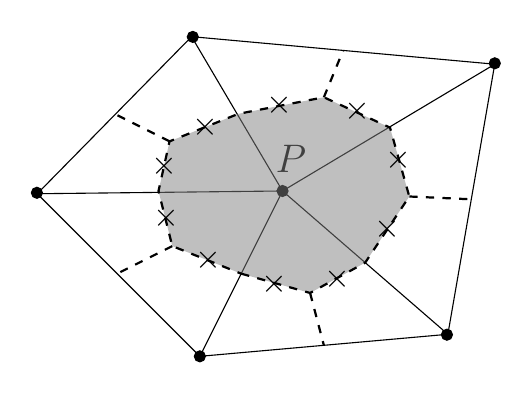
\begin{tikzpicture}[scale=3.5]
        % Generated with mktridual.py
\draw[] (0.00,0.00) -- (0.90,0.08) -- (1.07,1.06) -- (-0.03,1.16) -- (-0.59,0.59) -- cycle;
\draw [fill] (0.0, 0.0) circle [radius=0.02] node [] {};
\draw [fill] (0.896575228282571, 0.07844016847289235) circle [radius=0.02] node [] {};
\draw [fill] (1.0702234059495015, 1.0632479214851003) circle [radius=0.02] node [] {};
\draw [fill] (-0.025590761951418628, 1.1591192385075249) circle [radius=0.02] node [] {};
\draw [fill] (-0.5912761869006568, 0.5934338135582868) circle [radius=0.02] node [] {};
\draw [fill] (0.3, 0.6) circle [radius=0.02] node [above=3pt,xshift=3pt] {\Large $P$};
\draw[] (0.30,0.60) -- (0.00,0.00);
\draw[] (0.30,0.60) -- (0.90,0.08);
\draw[] (0.30,0.60) -- (1.07,1.06);
\draw[] (0.30,0.60) -- (-0.03,1.16);
\draw[] (0.30,0.60) -- (-0.59,0.59);
\draw[dashed,thick] (0.40,0.23) -- (0.45,0.04);
\draw[dashed,thick] (0.76,0.58) -- (0.98,0.57);
\draw[dashed,thick] (0.45,0.94) -- (0.52,1.11);
\draw[dashed,thick] (-0.11,0.78) -- (-0.31,0.88);
\draw[dashed,thick] (-0.10,0.40) -- (-0.30,0.30);
\draw[fill=gray,fill opacity=0.5,dashed,thick] (0.15,0.30) -- (0.40,0.23) -- (0.60,0.34) -- (0.76,0.58) -- (0.69,0.83) -- (0.45,0.94) -- (0.14,0.88) -- (-0.11,0.78) -- (-0.15,0.60) -- (-0.10,0.40) -- (0.15,0.30);
\node at (0.27,0.26) {\large $\times$};
\node at (0.50,0.28) {\large $\times$};
\node at (0.68,0.46) {\large $\times$};
\node at (0.72,0.71) {\large $\times$};
\node at (0.57,0.89) {\large $\times$};
\node at (0.29,0.91) {\large $\times$};
\node at (0.02,0.83) {\large $\times$};
\node at (-0.13,0.69) {\large $\times$};
\node at (-0.12,0.50) {\large $\times$};
\node at (0.03,0.35) {\large $\times$};

% \node [align=left] at (0.0, -0.3) {
%     \begin{tabular}{cl}
%     $\times$ & Integration point\\
%     \tikz\draw[fill] circle (0.5ex); & Field point
%     \end{tabular}
% };
    \end{tikzpicture}
    \caption{Dual control volume of a cell-vertex scheme in two dimensions. Integration surfaces are shown as dashed lines, the CV around $P$ is filled in gray, elements are separated by solid lines, the field point is shown as a solid black circle and integration points are shown as crosses.}
    \label{fig:dualmeshtwo}
\end{figure}

In three dimensions, sectors are generated by joining the element centroid to the element face centers, in combination with lines joining element face centers to the mid-points of the element edges. Again, the sub-division of an element yields as many sectors as vertices on the element.

The terminology introduced here will be used for the remainder of this work of~\Cref{sec:nxflow}. It should also be noted that ``vertex'' and ``node'' are used interchangeably.

\subsection{Control-volume based finite element method}
\label{sec:cvfem}
%
The CVFE method was first proposed by Baliga and Patankar in~\cite{baliga1980new,baliga1983control}. This new method borrows two characteristics from the finite element method (FEM):
\begin{enumerate}
    \item the use of element-based linear Lagrangian interpolation functions (shape functions)
    \item an element-by-element compilation of the coefficients in the discretized equations
\end{enumerate}
These two characteristics are briefly discussed in the following sections. Readers interested in a thorough discussion of the classical FEM applied to fluid flow problems are referred to~\cite{reddy2000finite}.

\subsubsection{Shape functions}
The shape functions $\shape$ represent the variation of solution inside an element. This allows one to calculate the value of a field variable $\phi$ at an $(s,t,u)$ coordinate within the element as follows:
\begin{equation*}
    \phi(s, t, u) = \sum_n^N \shape(s, t, u)_n\phi_n,
\end{equation*}
\begin{figure}
    \centering
    \begin{tikzpicture}[scale=4.0]
        \draw [fill] (0.0, 0.0) circle [radius=0.01] node [below] {1};
\draw [fill] (1.0, 0.0) circle [radius=0.01] node [below] {2};
\draw [fill] (1.0, 1.0) circle [radius=0.01] node [above] {3};
\draw [fill] (0.0, 1.0) circle [radius=0.01] node [above] {4};
\draw[dashed] (0.50,0.00) -- (0.50,0.50);
\node at (0.50,0.25) { $\times$};
\draw[dashed] (1.00,0.50) -- (0.50,0.50);
\node at (0.75,0.50) { $\times$};
\draw[dashed] (0.50,1.00) -- (0.50,0.50);
\node at (0.50,0.75) { $\times$};
\draw[dashed] (0.00,0.50) -- (0.50,0.50);
\node at (0.25,0.50) { $\times$};
\draw[] (0.00,0.00) -- (1.00,0.00) -- (1.00,1.00) -- (0.00,1.00) -- cycle;
\draw [thick, <->] (0.20,0.00) node [below right] {$s$} -- (0.00,0.00) -- (0.00,0.20) node [left] {$t$};
\draw [very thick, ->] (1.3, 0.5) -- (1.7, 0.5);
\draw [fill] (2.0, 0.0) circle [radius=0.01] node [below] {1};
\draw [fill] (2.8, 0.0) circle [radius=0.01] node [below] {2};
\draw [fill] (2.9, 1.1) circle [radius=0.01] node [above] {3};
\draw [fill] (2.05, 1.0) circle [radius=0.01] node [above] {4};
\draw[dashed] (2.40,0.00) -- (2.44,0.53);
\node at (2.42,0.26) { $\times$};
\draw[dashed] (2.85,0.55) -- (2.44,0.53);
\node at (2.64,0.54) { $\times$};
\draw[dashed] (2.47,1.05) -- (2.44,0.53);
\node at (2.46,0.79) { $\times$};
\draw[dashed] (2.02,0.50) -- (2.44,0.53);
\node at (2.23,0.51) { $\times$};
\draw[] (2.00,0.00) -- (2.80,0.00) -- (2.90,1.10) -- (2.05,1.00) -- cycle;
\draw [thick, <->] (2.16,0.00) node [below right] {$s$} -- (2.00,0.00) -- (2.01,0.20) node [left] {$t$};

    \end{tikzpicture}
    \caption{General linear quadrilateral element (right) and its representation in the natural coordinate system (left)}
    \label{fig:naturalcsys}
\end{figure}
where $N$ is the number of nodes in the element, $\phi_n$ is the stored value of $\phi$ at node $n$. The $s,t,u$ coordinate system is local to each element and is also referred to as the natural coordinate system in the FEM literature. Construction of shape functions in the $x,y,z$ coordinate system results in complex algebraic expressions, which is why it is best to express them in terms of the natural coordinates. Moreover, the integration point locations for a given element type will always be at the same $s,t,u$ coordinates. Values of $s,t,u$ are only allowed to vary between 0 and 1. The natural coordinate system transformation is illustrated in~\Cref{fig:naturalcsys} for a quadrilateral element (two-dimensional). For such an element, the shape functions can be written as:
\begin{align*}
    \shape_1(s,t) &= (1-s)(1-t)\\
    \shape_2(s,t) &= s(1-t)\\
    \shape_3(s,t) &= st\\
    \shape_4(s,t) &= (1-s)t.
\end{align*}
It is then straightforward to obtain the shape function derivatives with respect to local coordinates, which are given by:
\begin{equation*}
    \pdiff{\phi}{s_i} = \sum_n^N \pdiff{\shape_n}{s_i}\phi_n,
\end{equation*}
where $s_i$ represents the $i$-th component in the natural coordinate system. 

Similarly to the generalized curvilinear coordinates, a transformation is necessary to calculate the shape function derivatives with respect to the global coordinates $x,y,z$. The position vector can be expressed as a function of the $s,t,u$ coordinates as:
\begin{equation*}
    \vec{x}(s,t,u) = \sum_n^N \shape(s,t,u)_n\vec{x}_n.
\end{equation*}
This leads to the following metric formulation:
\begin{equation}
    \left.\pdiff{\vec{x}}{s_j}\right|_{(s,t,u)} = 
        \sum_n^N \left(\left.\pdiff{\shape_n}{s_j}\right|_{(s,t,u)} \vec{x}_{n}\right).
\end{equation}

The derivatives of $\phi$ with respect to the natural coordinates can be written in the following matrix form using the chain rule:
\begin{equation*}
    \begin{pmatrix}
        \pdiff{x}{s} & \pdiff{y}{s} & \pdiff{z}{s} \\
        \pdiff{x}{t} & \pdiff{y}{t} & \pdiff{z}{t} \\
        \pdiff{x}{u} & \pdiff{y}{u} & \pdiff{z}{u}
    \end{pmatrix}
    \begin{bmatrix}
        \pdiff{\phi}{x} \\
        \pdiff{\phi}{y} \\
        \pdiff{\phi}{z}
    \end{bmatrix}
    = 
    \begin{bmatrix}
        \pdiff{\phi}{s} \\
        \pdiff{\phi}{t} \\
        \pdiff{\phi}{u}
    \end{bmatrix}.
\end{equation*}
This system can be numerically inverted using Kramer's rule. 
The derivative $\partial \phi/\partial x$ at an integration point in the element can then be written as:
\begin{equation*}
    \left.\pdiff{\phi}{x_i}\right|_{ip} = \sum_n^N \left.\pdiff{\shape_n}{x_i}\right|_{ip}\phi_n.
\end{equation*}
It should be noted that the evaluation of $\phi$ and its derivative inside an element can be computed with second-order accuracy regardless of the shape of the element, which is a significant advantage of using this method -- the approximations in~\Cref{sec:syn3d} are at most second-order accurate, depending on the skewness and orthogonality of the grid.
 

\subsubsection{Compilation of the coefficients}
The CVFE method uses the integral form of the equations as discussed in~\Cref{sec:fv}, and fluxes through the integration surfaces around a control volume must be evaluated. Due to the dual mesh configuration, the integration surfaces as well as the integration points lie completely inside the elements. The surface integrals can then be calculated element-wise and accumulated to each control volume appropriately. The surface integrals are then guaranteed to be conservative. Moreover, because of the way the shape functions are constructed, the value of the flux at a given integration point depends on the field variables at all nodes in that element, regardless of whether the integration point belongs to their control volume. In other words, the stencil involved in the computation of a flux always includes all the vertices of the element in which the flux is computed.

It should be noted that boundaries of the domain require special treatment, since the surfaces are not located inside any element. This is discussed further below.

\subsection{Pressure-based solver}
\label{sec:pbased}
The main difference between a density-based and a pressure-based solver is the dependent variable in the mass equation, which is density in the former and pressure in the latter. Because a large portion of users of NX Flow want to simulate flows involving liquids, which have a constant density, the developers of NX Flow chose the pressure-based approach. In the case of ideal gases, the density is updated using the ideal gas law at each iteration.

NX Flow employs the collocated variables approach, i.e. pressure and velocity are stored at the same locations, proposed by Rhie and Chow~\cite{rhie1983numerical} in order to avoid pressure checkerboarding.

\subsection{Discretization of the governing equations}
\label{sec:nxnum}
This section describes the numerical discretization of the terms in the mass, momentum, energy and turbulence equations. 

NX Flow being a commercial code, offers a wide variety of options to its users. For the sake of conciseness, only the options used to solve the problems in this work are described. 

\subsubsection{Temporal discretization}
NX Flow uses the fully-implicit first-order backward Euler approach to discretize the time derivative of all partial differential equations. It solves the mass and momentum equations together, which yields an updated pressure and velocity field. 

%In the case of the conservation laws, this leads to a coupled system of five equations for each control volume:
%\begin{equation*}
%    \left[
%        \frac{V}{\Delta t^n} - \pdiff{\vec{R}^n}{\vec{W}}
%    \right] \Delta \vec{W}^n = \vec{R}^n
%\end{equation*}
%where $\vec{W}$ is defined in~\Cref{eq:wstate}. 

The turbulence and energy equations are not coupled with the mass and momentum equations; they are solved separately in a segregated manner. The linear systems are solved using an iterative solver such as GMRES.

\subsubsection{Discretization of convective fluxes}
The convective flux of an arbitrary quantity over an integration surface can be written in the following general form:
\begin{equation*}
    \int_S (\rho\vec{u}\phi)\cdot\vec{n}~dS = \dot{m}_{ip}\phi_{ip},
\end{equation*}
where $\dot{m}_{ip}$ is the mass flow rate through the integration surface and is evaluated using the shape functions along with a pressure correction term~\cite{schneider1987control,rhie1983numerical}. The method is actually slightly modified from the cited references, but cannot be discussed.

The value of $\phi$ at the integration point also needs to be approximated in terms of the nodal values of $\phi$. The default scheme for this is a first-order upwind scheme, in which $\phi_{ip}$ is approximated by the value of $\phi$ at the upstream node, i.e.:
\begin{equation*}
    \phi_{ip} = \phi_{i},
\end{equation*}
where the upstream node is determined using the sign of the mass flux. This scheme leads to a stable and quick convergence at the expense of reduced accuracy.

\subsubsection{Discretization of viscous fluxes}
Computation of the diffusive fluxes requires evaluation of the diffusion coefficient and spatial derivatives at the integration points. This is simply done using the finite element shape functions. The gradient and diffusion coefficient at an integration point are then evaluated as:
\begin{align*}
    \Gamma_{ip} &= \sum_n^N \left.\shape_n\right|_{ip}\Gamma_n \\
    \left.\nabla\phi\right|_{ip} &= \sum_n^N \left.\nabla\shape_n\right|_{ip}\phi_n.
\end{align*}

\subsubsection{Discretization of pressure term}
The pressure gradient term is treated as a surface force via the divergence theorem, similarly to syn3D. The value of pressure must then be evaluated at all integration points, which is done using the shape functions.

\subsubsection{Discretization of nodal gradients}
Source terms sometimes require the computation of gradients at field points, as opposed to at an integration point. Such nodal gradients can also be computed using a form of the divergence theorem. The gradient of $\phi$ at node $P$ can then be computed as follows:
\begin{equation*}
    (\nabla \phi)_P = \frac{1}{V}\sum_{ip}(\phi\vec{n})_{ip}.
\end{equation*}
The formula requires that $\phi$ be evaluated at integration points, which is done using the shape functions.

\subsubsection{Boundary conditions}
NX Flow was unfortunately not developed with external flows in mind and does not offer far-field boundary conditions in its catalogue. The user must then use internal flow BCs such as inlets and openings. The following boundary conditions are used in this work:
\begin{itemize}
    \item Solid wall
    \item Inlet
    \item Opening
    \item Symmetry plane
\end{itemize}
Treatment of boundary conditions in a vertex-centered code is quite different from that of a cell-centered code since some field points may lie on the boundary, as depicted in~\Cref{fig:cvfebc}. Such points have integration surfaces corresponding to segments of the boundary. It should be noted that evaluation of fluxes over the domain then requires two loops: one over the elements and the interior integration surfaces as well as one over the boundary integration surfaces. 
\begin{figure}
    \centering
    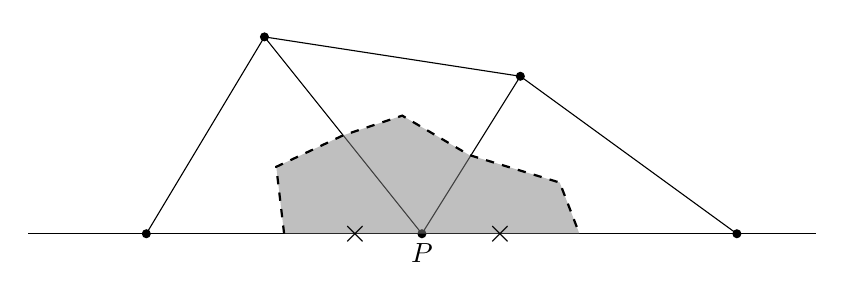
\begin{tikzpicture}[scale=5.0]
        \draw[thin] (-1.00,0.00) -- (1.00,0.00);
\draw [fill] (-0.7, 0.0) circle [radius=0.01] node [] {};
\draw [fill] (0.0, 0.0) circle [radius=0.01] node [below] {$P$};
\draw [fill] (0.8, 0.0) circle [radius=0.01] node [] {};
\draw [fill] (-0.4, 0.5) circle [radius=0.01] node [] {};
\draw [fill] (0.25, 0.4) circle [radius=0.01] node [] {};
\draw[] (-0.70,0.00) -- (0.00,0.00);
\draw[] (-0.70,0.00) -- (-0.40,0.50);
\draw[] (0.00,0.00) -- (0.80,0.00);
\draw[] (0.00,0.00) -- (-0.40,0.50);
\draw[] (0.00,0.00) -- (0.25,0.40);
\draw[] (0.80,0.00) -- (0.25,0.40);
\draw[] (-0.40,0.50) -- (0.25,0.40);
\draw[fill=gray,opacity=0.5,draw=none] (-0.35,0.00) -- (-0.37,0.17) -- (-0.20,0.25) -- (-0.05,0.30) -- (0.12,0.20) -- (0.35,0.13) -- (0.40,0.00) -- cycle;
\draw[dashed,thick] (-0.35,0.00) -- (-0.37,0.17) -- (-0.20,0.25) -- (-0.05,0.30) -- (0.12,0.20) -- (0.35,0.13) -- (0.40,0.00);
\node at (-0.17,0.00) {\large $\times$};
\node at (0.20,0.00) {\large $\times$};
    \end{tikzpicture}
    \caption{Control volume for a boundary vertex $P$. Only boundary integration points are shown.}
    \label{fig:cvfebc}
\end{figure}

Symmetry planes require that there be no flux through the boundary. The implementation of such a boundary condition simply requires not calculating any fluxes through the boundary integration surfaces. 

In an inlet BC, the user specifies values for velocity and its direction as well as pressure, temperature and turbulence quantities. Since the integration point is on the boundary, convective and diffusive fluxes can be calculated using the user-specified values as the $ip$ values, i.e. no interpolation is required. The gradients are calculated using the shape function derivatives, except that the node values are replaced with the integration point values for nodes on the boundary. The gradient of $\phi$ at a boundary integration point $ip,b$ can then be expressed as a sum over the interior nodes, the ones not on a boundary, and boundary nodes:
\begin{equation*}
    \left.\nabla\phi\right|_{ip,b} = \sum_{interior}\left.
        \nabla\shape_n\right|_{ip,b}
    \phi_n + \sum_{boundary}\left.
        \nabla\shape_n\right|_{ip,b}
    \phi_{ip,b}.
\end{equation*}

Opening BCs specify pressure, temperature and turbulence quantities. The velocity at boundary integration points is obtained by shape function interpolation, which determines whether the opening is an inflow or outflow. The advection term requires no special treatment. On the other hand, the diffusion flux is only calculated if the flow is outgoing. All openings used in this work should be treated as outflows.

Viscous wall boundary conditions can be implemented strongly by directly imposing prescribed values at the nodes (Dirichlet) or weakly by instead imposing a condition on the flux through specification of $\phi_{ip,b}$. A detailed discussion can be found in~\cite{nordstrom2012weak}. This BC is currently implemented weakly for the mass and momentum and strongly for the turbulence equations. 

\subsection{Wall distance calculation}
\label{sec:nxwalldist}
NX Flow also offers both the brute force approach and Poisson approach to calculate the wall distance. The brute force approach finds the nearest node for every field point, and the Poisson equation is solved with the finite volume method, exactly like the Navier-Stokes equations. 
